%
%  final-report.tex
%  Desktop
%
%  Created by Illya Starikov on 11/20/17.
%  Copyright 2017. Illya Starikov. All rights reserved.
%

\RequirePackage[l2tabu, orthodox]{nag}
\documentclass[12pt,titlepage=false]{scrartcl}

\usepackage{amssymb,amsmath,verbatim,graphicx,microtype,upquote,units,booktabs,siunitx,xcolor,multicol,pdfpages,float,array,wrapfig,titlesec,subcaption}

\newcommand{\sectionbreak}{\clearpage}
\setuptoc{toc}{leveldown}

\usepackage[english]{babel}
\DeclareSIUnit\quart{qt}
\DeclareSIUnit\tablespoon{tbsp}
\DeclareSIUnit\cup{cup}

\usepackage{caption}
\captionsetup[table]{skip=2pt}
\setlength{\tabcolsep}{5pt}

\title{Project Report}
\subtitle{STAT 3113 --- Engineering Statistics}
\date{Due Date: November 30\textsuperscript{th}, 2017}
\author{Caroline Ketterer, Sam McGraw, Illya Starikov, Timothy Ott}

\begin{document}
\maketitle
\tableofcontents

\section{Objective}
A useful tool in cooking is determining roughly how long it will take to boil water. There are several factors that might affect how fast water boils, including:

\begin{itemize}
    \item Amount of salt in the water.
    \item The size of the pot.
\end{itemize}

This experiment will specifically determine how said factors affect how long it takes water to reach \SI{100}{\degreeCelsius}.

\section{Experiment Design}
\label{sec:experiment_design}
Below we will lay out the design of our experiment.

\subsection{Factors and Levels}
\label{sub:factors_and_levels}
We design a two factor, three level experiment --- a $3^2$ factorial experiment. Please refer to Table~\ref{tab:factors_levels} for a complete description.

\begin{table}[H]
    \centering
    \caption{Factor and Level Definition}
    \label{tab:factors_levels}
    \begin{tabular}{cccc}
        \toprule
        \textbf{Factor} & \textbf{Level 1} & \textbf{Level 2} & \textbf{Level 3} \\\hline
        \textit{Pan Size} & \SI{153.94}{\centi\meter\squared} & \SI{254.47}{\centi\meter\squared} & \SI{314.16}{\centi\meter\squared} \\
        \textit{Salt Weight} & No Salt & \SI{17}{\gram} & \SI{34}{\gram} \\
        \bottomrule
    \end{tabular}
\end{table}

\subsection{Response Variable}
\label{sub:response_variable}
In our experiment, the response variable is the amount of time it takes for two cups of water to reach \SI{100}{\degreeCelsius}.

\subsection{Blocking Factors}
\label{sub:blocking_factors}
There is only one possible blocking factor for our experiment: the initial temperature of the pot. We circumvent this by placing cold water in all of the pans initially and letting all the pans reach thermal equilibrium before starting the experiment.

\subsection{Number of Replicants}
\label{sub:number_of_replicants}
Each treatment combination is replicated three times.

\section{Experiment Plan}
\label{sec:experiment_plan}
The following section will describe the layout of the experiment.

\subsection{Letting Pans Reach Thermal Equilibrium}
\label{sub:letting_pans_reach_thermal_equilibrium}

The first step is to ensure that all pans have the same initial temperature.

We accomplish this by placing cold water (\SI{5}{\degreeCelsius}) in both of the pans for 5:00 minutes. After this, we can proceed with the experiment.

\subsection{Measure Out Salt}
\label{sub:measure_out_salt}
\begin{wrapfigure}{r}{0.5\textwidth}
    \begin{center}
        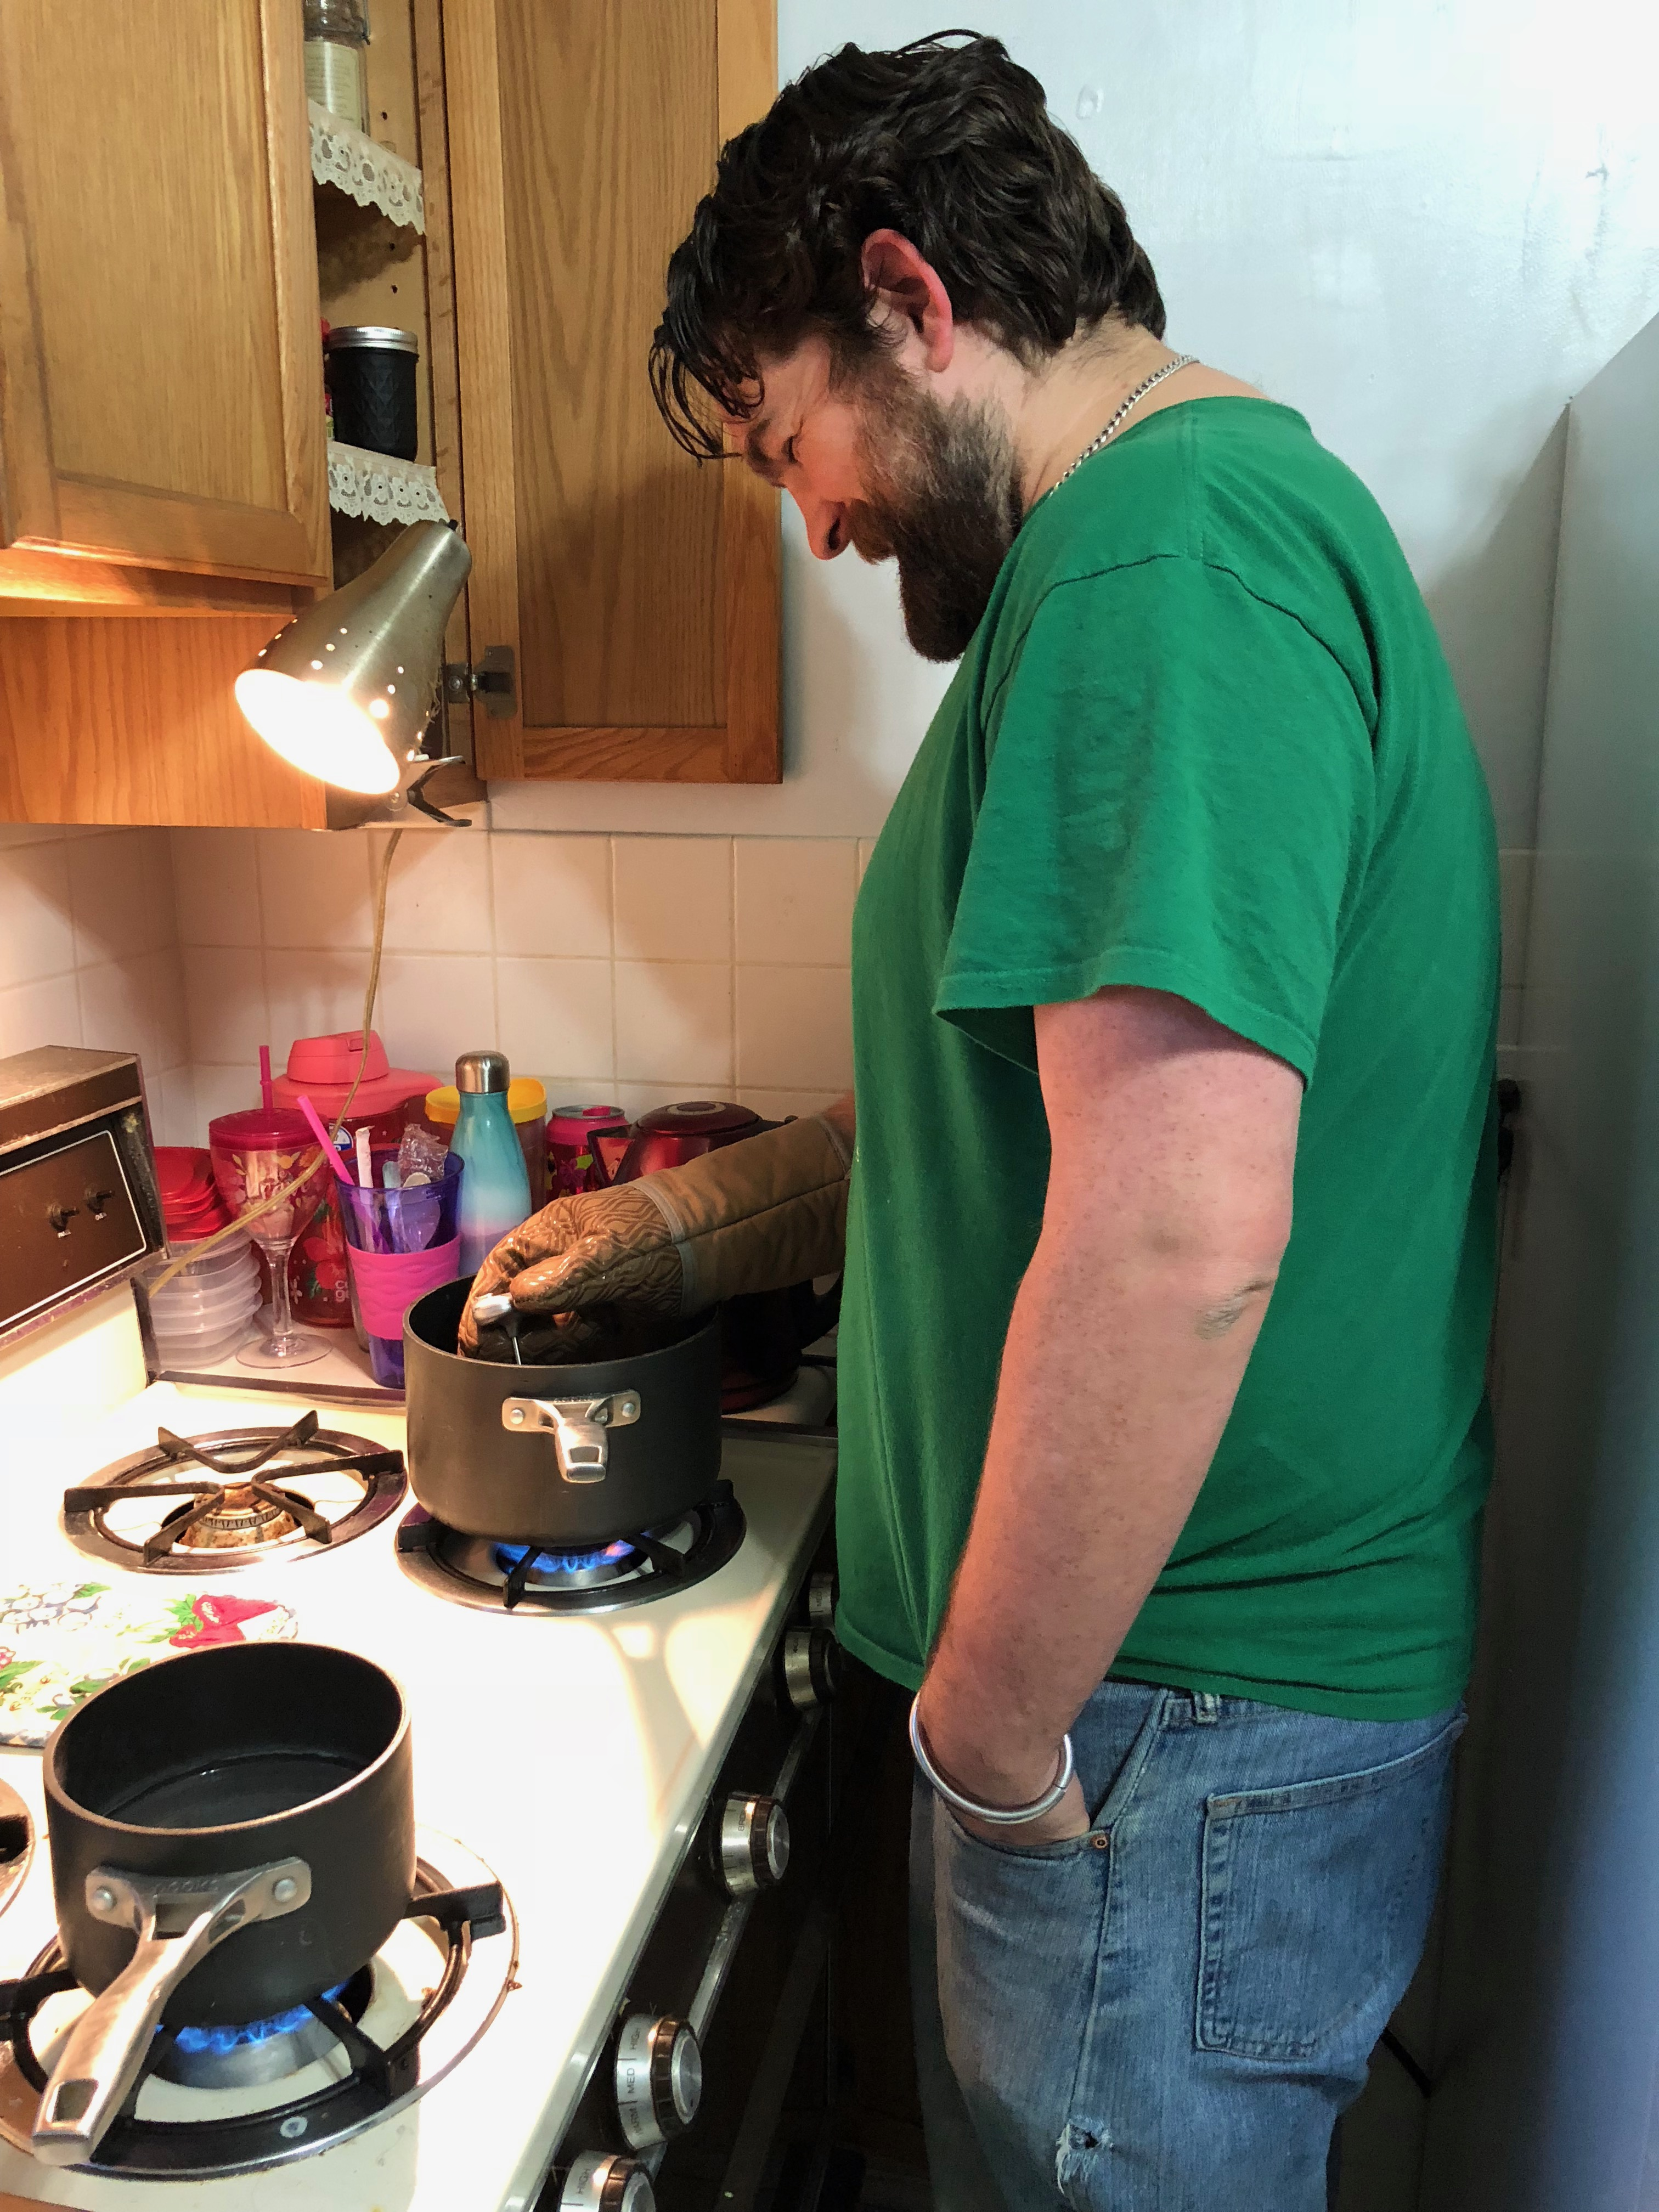
\includegraphics[width=0.30\textwidth]{tim}
    \end{center}
    \caption{Timothy Ott Conducting The Experiment}
\end{wrapfigure}

\textit{Note: This step does not apply to the treatment with no salt.}

We measure out the salt on a scale to the desired weight (whether it be \SI{17}{\gram} or \SI{34}{\gram}).

After pouring said salt into all of the pans individually, we stir until we reach a homogeneous, saltwater mixture.

\subsection{Conduct The Experiment}
\label{sub:starting_heating_the_pots}

We proceed to set the temperature of all heating elements ``high''. We continually measure all pots to see if they have reached \SI{100}{\degreeCelsius}.

If they have reached the desired temperature, take the pot off the heater and mark the time. Do so for all pots.

After all pans have finished, mark the recorded data --- these notes can be found in Section~\ref{sec:appendix}

\section{Data Collection}
All data collected can be summarized Table~\ref{tab:data}; additionally, Section~\ref{sec:appendix} contains the data as it was collected during the experiment.

\begin{table}[H]
    \centering
    \caption{Number of Minutes To Reach \SI{100}{\degreeCelsius} (No Salt)}
    \label{tab:data}
    \resizebox{.95\linewidth}{!}{
        \begin{tabular}{r|ccc|ccc|ccc}
            \toprule
            & \multicolumn{3}{c|}{No Salt} & \multicolumn{3}{c|}{\SI{17}{\gram} Salt} & \multicolumn{3}{c}{\SI{34}{\gram} Salt} \\\hline
            \textbf{Big}    & 6:00.18 & 6:29.03 & 6:36.66 & 4:57.91 & 5:32.9 & 5:41.30 & 4:55.35 & 5:20.36 & 5:01.71 \\
            \textbf{Medium} & 7:36.48 & 5:41.17 & 6:56.42 & 5:22.78 & 6:17.04 & 5:55.60 & 5:33.12 & 5:34.46 & 5:35.75 \\
            \textbf{Small}  & 8:15.79 & 6:57.90 & 7:13.85 & 6:08.14 & 6:34.02 & 6:47.33 & 6:03.25 & 6.08.36 & 6:04.19 \\
            \bottomrule
        \end{tabular}
    }
\end{table}

\section{Data Analysis}
\label{sec:data_analysis}
We entered the data of our experiment into the JMP software as shown below. The data can be viewed in Figure\ref{fig:inputs}

\begin{figure}[H]
    \centering
    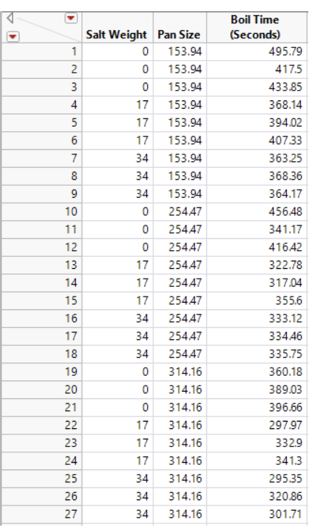
\includegraphics[width=0.5\linewidth]{inputs}
    \caption{The Input Used By JMP.}
    \label{fig:inputs}
\end{figure}

To analyze the data we first needed to test for the presence of interaction effect.

\begin{align*}
    H_0&: \gamma_{11} = \gamma_{12} = \ldots = \gamma_{IJ} = 0 \\
    H_1&: \text{at least one of the $\gamma_{ij}$ is nonzero}
\end{align*}

Because the $p$-value of Salt Water*Pan Size is \num{0.7625} (Figure~\ref{fig:results}), which is greater than our significance level of \num{0.05}, we fail to reject our null hypothesis and conclude that the interaction effect is not significant. Therefore, we can test for the main effects.

\begin{figure}[t!]
    \begin{subfigure}[t]{0.45\textwidth}
        \begin{center}
            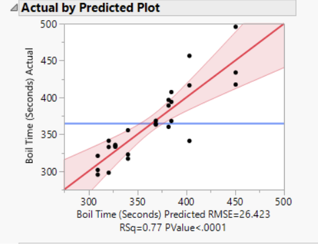
\includegraphics[width=\textwidth]{actual-by-predicted-plot.png}
        \end{center}
        \caption{The Actual by Predicted Plot}
    \end{subfigure}
    ~
    \begin{subfigure}[t]{0.45\textwidth}
        \begin{center}
            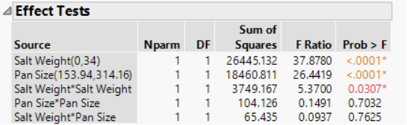
\includegraphics[width=\textwidth]{effects.png}
        \end{center}
        \caption{The Main Effects Table}
    \end{subfigure}

    \caption{The Results}
    \label{fig:results}
\end{figure}

\section{Conclusion}
\label{sec:conclusion}
To test the main effects we first need to define our null and alternative hypotheses. We will first consider pan size.

\begin{align*}
    H_0&: \alpha_1 = \alpha_2 = \ldots = \alpha_I = 0 \\
    H_1&: \text{at least one of the $\alpha_i$ is nonzero}
\end{align*}

The $p$-value for pan size is a number smaller than \num{0.0001} which is smaller than our significance level of \num{0.05}. Therefore, we fail to reject our null hypothesis and conclude that pan size does have an effect on the time it takes for water to reach \SI{100}{\degreeCelsius}.

We will now test for the main effect of salt weight.

\begin{align*}
    H_0&: \beta_1 = \beta_2 = \ldots = \beta_J = 0 \\
    H_1&: \text{at least one of the $\beta_j$ is nonzero}
\end{align*}


The $p$-value for salt weight is a number smaller than \num{0.0001} which is again smaller than our significance level of \num{0.05}. Therefore, we fail to reject our null hypothesis and conclude than salt weight does have an effect on the time it takes for water to reach \SI{100}{\degreeCelsius}.

\section{Improvement Suggestions}
\label{sec:improvement_suggestions}
There are still things that can be improved in our experiment; specifically, they are:

\begin{description}
    \item[Filtered Water] Using filtered water, as opposed to tap water, would also improve the accuracy of the experiment.  Tap water naturally contains various minerals, ions, and other particles that vary greatly between samples.  Filtered water would remove the interference of those particles, making the salt the only additive in the water.

    \item[Better Temperature Measurement] Creating a rig to hold the thermometer in the water would also improve the accuracy of our results.  Manually dipping the thermometer between the pots adds some variation between measurements, while having some method for holding the thermometer in the center of the pot would ensure consistent, unbiased results.

    \item[Atmospheric Pressure] Controlling the atmospheric pressure at which the experiment was conducted would improve the accuracy of this experiment.  The air pressure above the water changes the temperature/amount of time required to boil water, and since this experiment took place over the course of several hours, the atmospheric pressure is liable to change.  Conducting the experiment in a controlled, pressurized environment would eliminate the variation in boiling pressures, thus producing consistent results.
\end{description}

\section{Appendix}
\label{sec:appendix}
The following are notes collected from the experiment.

\begin{multicols}{2}
    \centering
    \frame{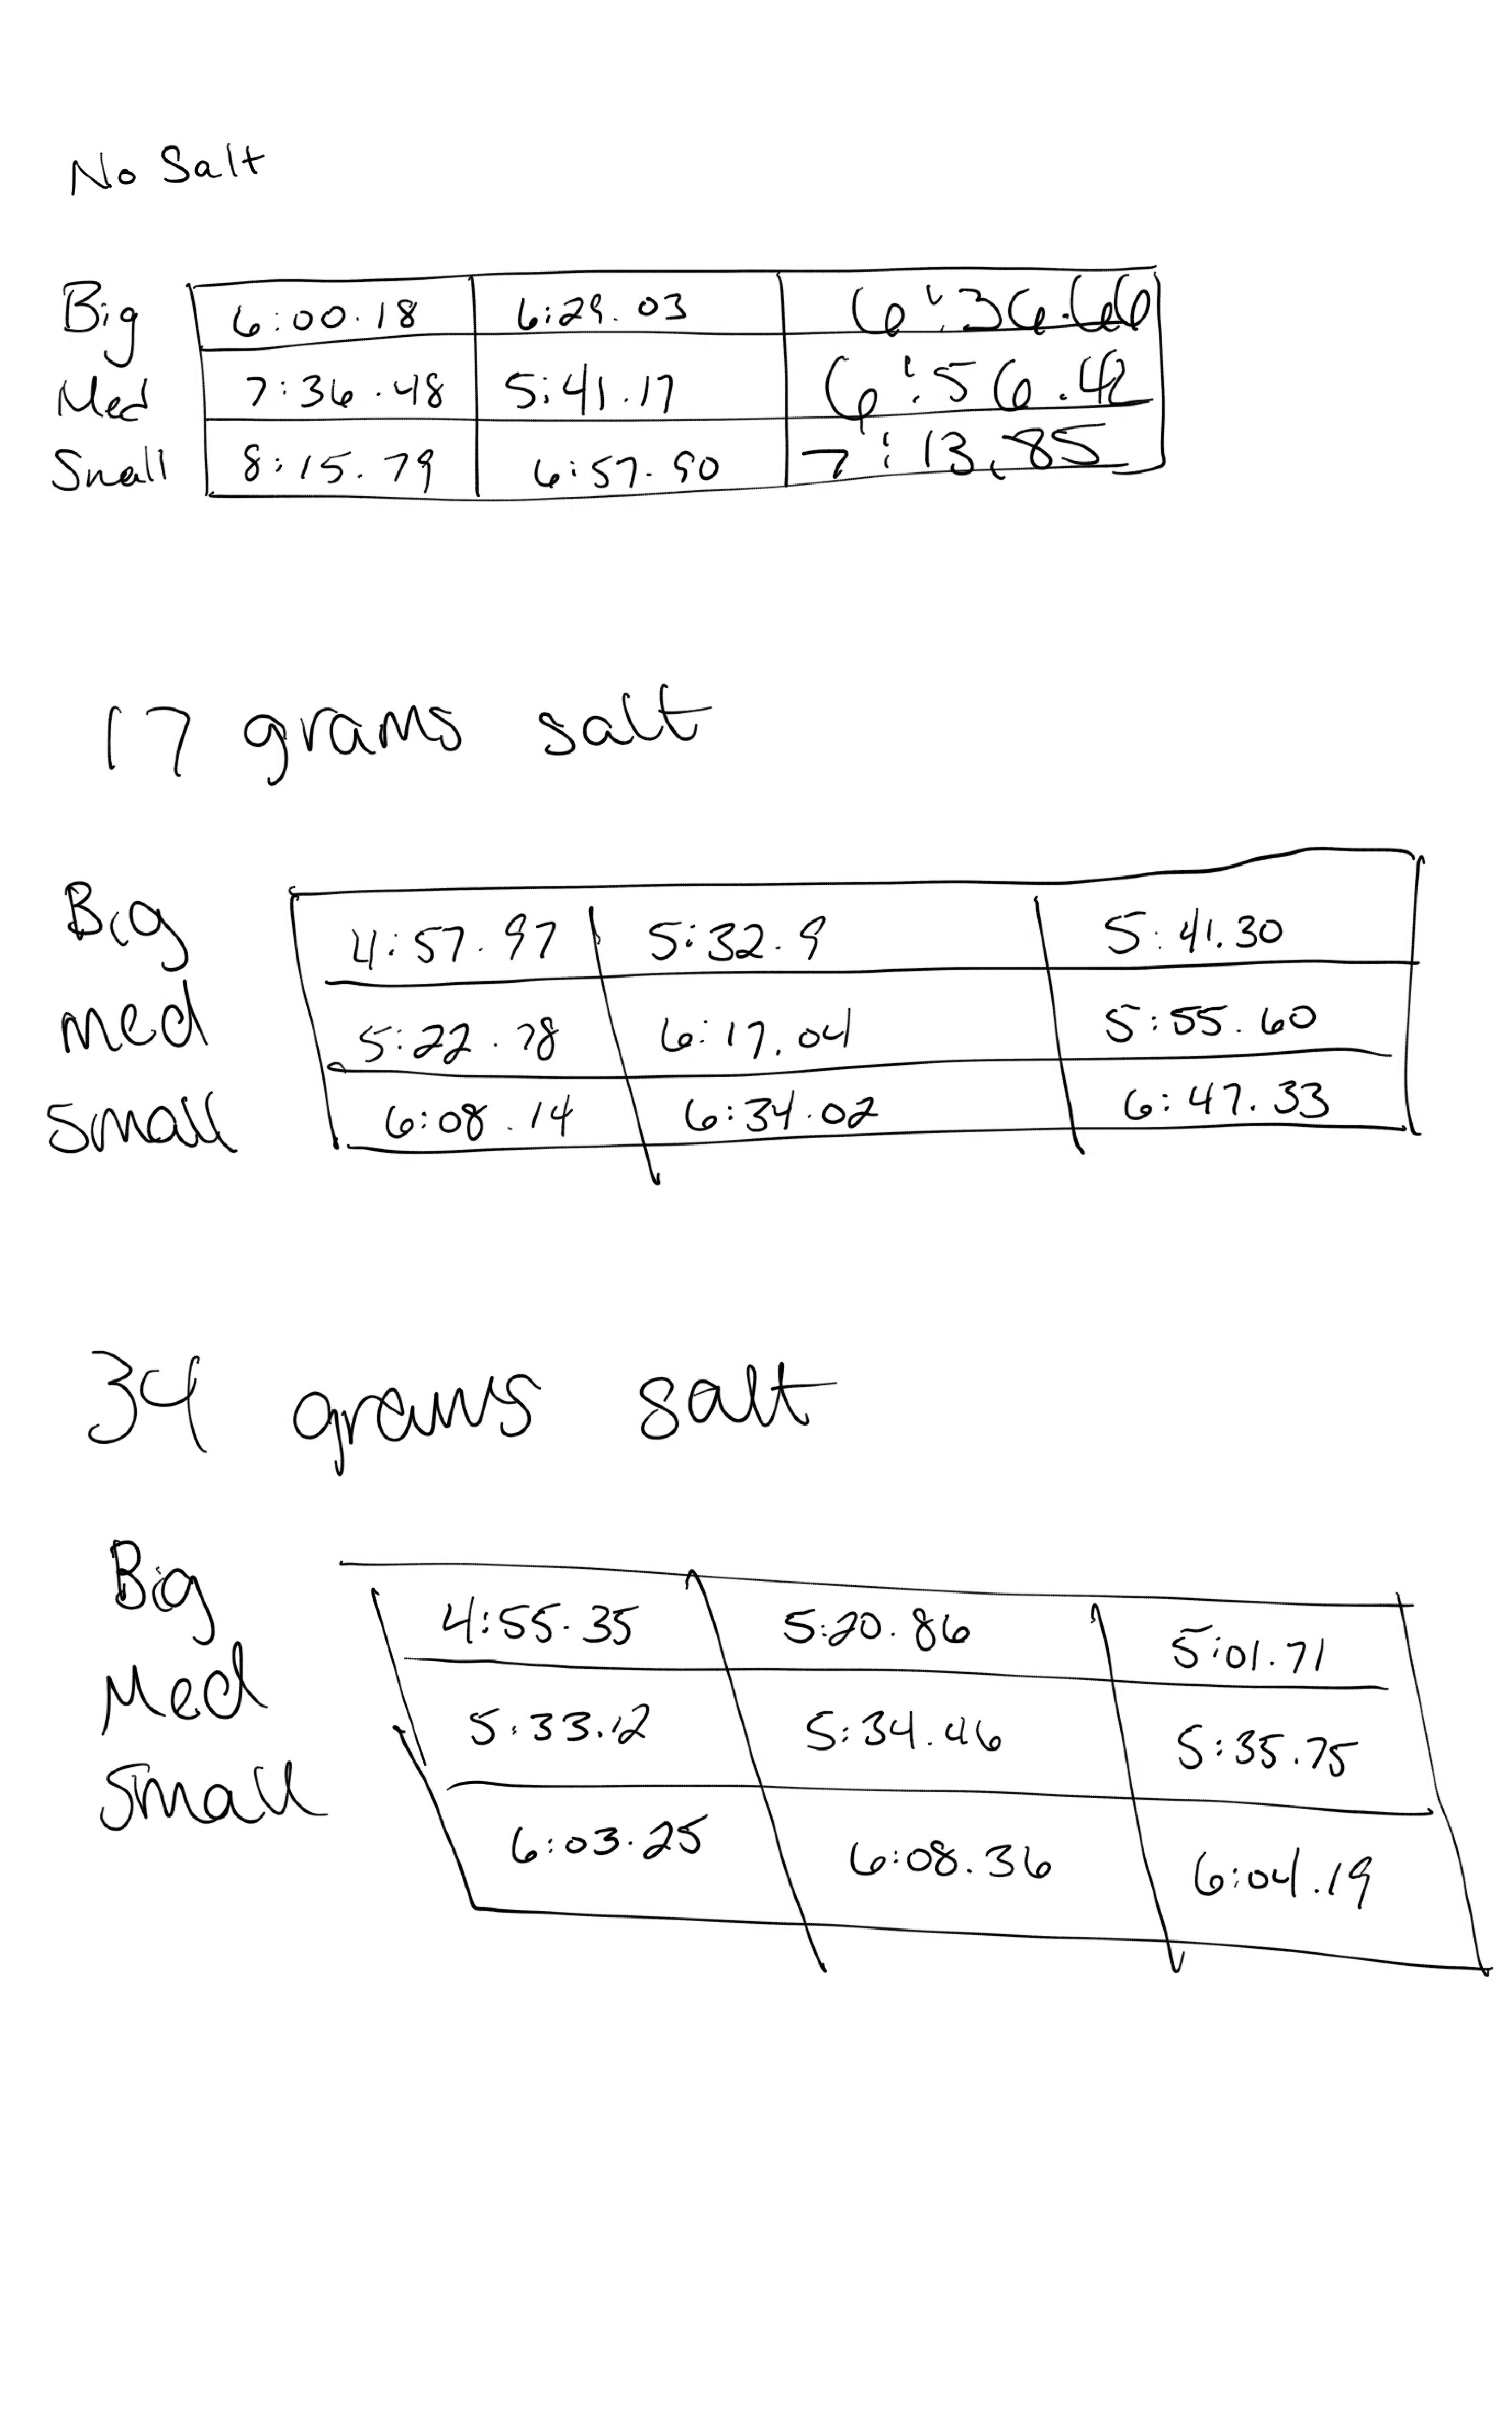
\includegraphics[width=.45\textwidth,page=1]{results.pdf}}
    \frame{\includegraphics[width=.45\textwidth,page=2]{results.pdf}}
\end{multicols}

\end{document}

